%!TEX root = ./trampoline.tex

\chapter{System generation and compilation}

Trampoline is a static operating system. This means all the objects (tasks, ISR, ...) are known at compile time. This way, an application is made of tasks' code and ISRs' code, application data, and statically initialized descriptor for each object the operating system manages. A system generation tool, like \goil, generates these descriptors in C files from an application configuration described in OIL or in XML. After that the Trampoline source code, the generated files and the application source code are compiled and linked together to produce an executable file as shown in figure \ref{fig:buildtrampoline}.

\begin{figure}[htbp] %  figure placement: here, top, bottom, or page
   \centering
   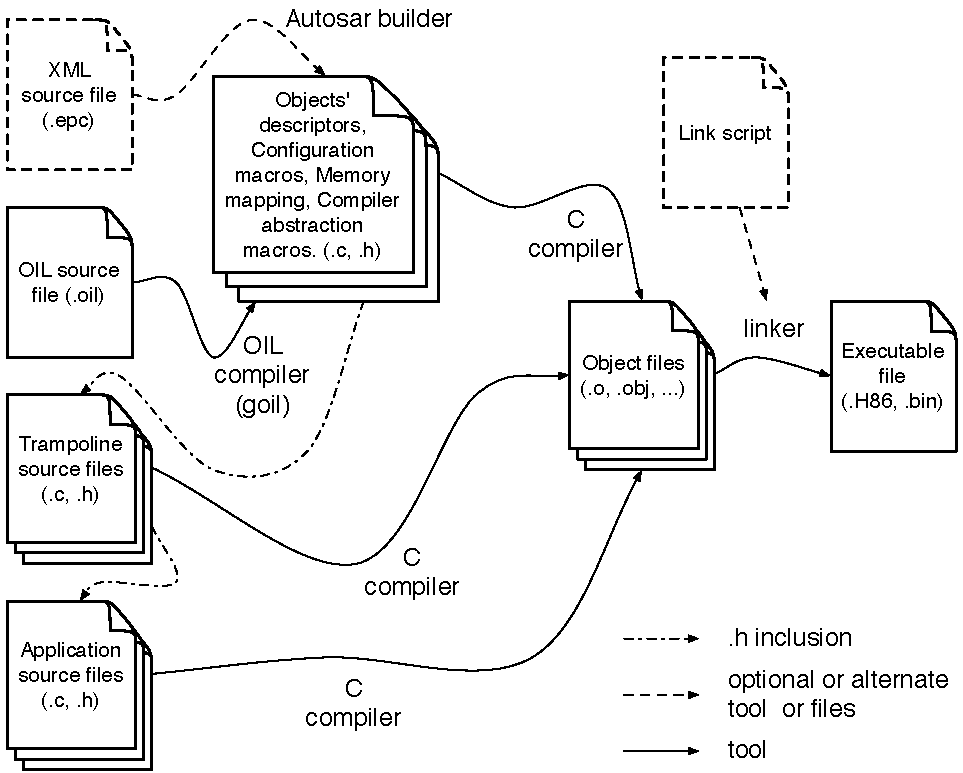
\includegraphics[width=4.5in]{pictures/buildProcess.pdf} 
   \caption{\textbf{Build process of an application with Trampoline.} Starting from the left, the .c and .h corresponding to the application description given in OIL (or XML) are generated by \goil\ (or another system generation tool, for instance an Autosar compliant one) and compiled using a C compiler. Trampoline source files are compiled too and include .h from the description for configuration purpose (see section \ref{sec:configmacros}). Application files are compiled and include .h files from Trampoline. All the object files are then linked together using an optional link script generated by \goil\ or provided with the application.}\label{fig:buildtrampoline}
\end{figure}

\section{The generated files}
\label{sec:generatedfiles}

The following files are generated by \goil\ from the OIL file or should be generated if you use a different system configuration tool. More information may be found in part \ref{part:goil}.

\rowcolors{1}{white}{light-gray}
\begin{longtableii}{l|p{3.5in}}{file}{File name}{Usage}

\lineii{tpl_app_define.h\index{tpl_app_define.h}}{This file contains all the configuration macros (see section \ref{sec:configmacros}) and is included in all the Trampoline files to trigger conditional compilation. \goil\ generates this file using the \file{tpl_app_define_h.goilTemplate} template file.}

\lineii{tpl_app_config.h\index{tpl_app_config.h}}{This file contains the declarations of the constants and functions required by the OSEK and Autosar standard (like OSMAXALLOWEDVALUE_x, OSTICKSPERBASE_x or OSMINCYCLE_x constants for counter x). \goil\ generates this file using the \file{tpl_app_config_h.goilTemplate} template file.}

\lineii{tpl_app_config.c\index{tpl_app_config.c}}{This file contains the definitions of the constants and functions required by the OSEK and Autosar standard and the definitions of object descriptors used by Trampoline (see section \ref{sec:structs}) \goil\ generates this file using the \file{tpl_app_config_c.goilTemplate} template file.}

\lineii{tpl_app_custom_types.h\index{tpl_app_custom_types.h}}{Some data types used by Trampoline are not statically defined. They are generated to fit size or performance criterions. For instance, the type used for a TaskType may be a byte if there is less than 256 tasks in the system and a word otherwise. This file defined these data types.}

\lineii{tpl_service_ids.h\index{tpl_service_ids.h}}{This file is generated only if Trampoline is compiled with service calls implemented using a system call. It contains all the identifiers of the services used by the application according to the configuration. \goil\ generates this file using the \file{tpl_service_ids_h.goilTemplate} template file.}

\lineii{tpl_dispatch_table.c\index{tpl_dispatch_table.c}}{This file is generated only if Trampoline is compiled with service calls implemented using a system call. It contains the dispatch table definition. See section \ref{sec:dispatchtable}. \goil\ generates this file using the \file{tpl_dispatch_table_c.goilTemplate} template file.}

\lineii{tpl_invoque.S\index{tpl_invoque.S}}{This file is generated only if Trampoline is compiled with service calls implemented using a system call. It contains the API functions for system services. See section \ref{sec:invoque}. The extension (here .S) may change according to the assembler used. \goil\ generates this file using the \file{tpl_invoque.goilTemplate} and \file{service_call.goilTemplate} template files.}

\lineii{MemMap.h\index{MemMap.h}}{This file is generated only if memory mapping is enabled. It contains macros for compiler abstraction memory mapping of functions and data as defined in the Autosar standard \cite{autosar31memorymapping}. \goil\ generates this file using the \file{MemMap_h.goilTemplate} template file.}

\lineii{Compiler.h\index{Compiler.h}}{This file is generated only if memory mapping is enabled. It contains macros for the compiler abstraction of functions and pointer qualifier as defined in the Autosar standard \cite{autosar31compilerabstraction}. \goil\ generates this file using the \file{Compiler_h.goilTemplate} template file.}

\lineii{Compiler_Cfg.h\index{Compiler_Cfg.h}}{This file is generated only if memory mapping is enabled. It contains macros for the compiler abstraction configuration as defined in the Autosar standard \cite{autosar31compilerabstraction}. \goil\ generates this file using the \file{Compiler_Cfg_h.goilTemplate} template file.}

\lineii{script.ld\index{script.ld}}{This file is generated only if memory mapping is enabled. It contains a link script to map the executable in the target memory. \goil\ generates this file using the \file{script.goilTemplate} template file.}

\end{longtableii}

The following sections give details about the content of these files.

\section{The Configuration Macros}
\label{sec:configmacros}

Trampoline can be compiled with various options. These options are controlled by setting the appropriate preprocessor configuration macros%
\index{Configuration macros}.
These macros are usually set by \goil
using the template found in \file{tpl_app_define_h.goilTemplate} file to produce the \file{tpl_app_define.h}\index{tpl_app_define.h} file that is included by the files of Trampoline. However, a different generation tool may be used and it should comply to the specification presented in the following tables. When Trampoline is compiled, the coherency and consistency of the configuration macros are checked, by using the preprocessor macros located in the \file{tpl_config_check.h} file, to ensure they correspond to a supported configuration.

3 kinds of configuration macros are used: boolean macros, numerical macros, symbol macros and string macros. Boolean macros may take 2 values: YES or NO. All macros should be defined, Trampoline does not use the \lstinline[language=C]{#ifdef} or \lstinline[language=C]{\#ifndef} scheme to limit the occurrences of unwanted misconfigurations except to prevent multiple inclusions of the same header file.

\subsection{Number of objects macros}

These macros gives the number of objects of each kind (tasks, ISRs, resources, \ldots) and other values. They are used in Trampoline to check the validity of the various identifiers and to define tables of the corresponding size:
 
\rowcolors{1}{white}{light-gray}
\begin{longtableiii}{l|l|p{3.1in}}{var}{Macro}{Kind}{Effect}
  \lineiii{\idxconfflag{PRIO_LEVEL_COUNT}}
  {Integer}
  {The number of priority levels used in the system.}
  \lineiii{\idxconfflag{TASK_COUNT}}
  {Integer}
  {The number of tasks (basic and extended) used in the system.}
  \lineiii{\idxconfflag{EXTENDED_TASK_COUNT}}
  {Integer}
  {The number of extended tasks used in the system.}
  \lineiii{\idxconfflag{ISR_COUNT}}
  {Integer}
  {The number of ISR category 2 used in the system.}
  \lineiii{\idxconfflag{ALARM_COUNT}}
  {Integer}
  {The number of alarms used in the system.}
  \lineiii{\idxconfflag{RESOURCE_COUNT}}
  {Integer}
  {The number of resources used in the system.}
  \lineiii{\idxconfflag{SEND_MESSAGE_COUNT}}
  {Integer}
  {The number of send messages used in the system.}
  \lineiii{\idxconfflag{RECEIVE_MESSAGE_COUNT}}
  {Integer}
  {The number of receive messages used in the system.}
  \lineiii{\idxconfflag{SCHEDTABLE_COUNT}}
  {Integer}
  {The number of schedule tables used in the system. This macros is only used when WITH_AUTOSAR is set to YES.}
  \lineiii{\idxconfflag{COUNTER_COUNT}}
  {Integer}
  {The number of counters used in the system. This macros is only used when WITH_AUTOSAR is set to YES.}
  \lineiii{\idxconfflag{APP_COUNT}}
  {Integer}
  {The number of OS applications used in the system. This macros is only used when WITH_AUTOSAR is set to YES.}
  \lineiii{\idxconfflag{TRUSTED_FCT_COUNT}}
  {Integer}
  {The number of trusted functions used in the system. This macros is only used when WITH_AUTOSAR is set to YES.}
  \lineiii{\idxconfflag{RES_SCHEDULER_PRIORITY}}
  {Integer}
  {The priority of the RES_SCHEDULER resource. This should be equal to the highest priority among the tasks.}
\end{longtableiii}

\subsection{Error Handling Macros}

Error handling related macros are used to configure what kind of error Trampoline checks and what extra processing is done when an error is encountered. The following macros are available:

\rowcolors{1}{white}{light-gray}
\begin{longtableiii}{l|l|p{2.5in}}{var}{Macro}{Kind}{Effect}
  \lineiii{\idxconfflag{WITH_OS_EXTENDED}}
  {Boolean}
  {When set to YES, Trampoline system services perform error checking on their arguments. \var{WITH_OS_EXTENDED} is set to YES with a \var{STATUS} = EXTENDED and is set to NO with a \var{STATUS} = BASIC in the oil OS object.}
  \lineiii{\idxconfflag{WITH_ERROR_HOOK}\label{sec:errorhook}}
  {Boolean}
  {When set to YES, the \function{ErrorHook()} function is called if an error occurs. \var{WITH_ERROR_HOOK} is set to YES/NO with a \var{ERRORHOOK} = TRUE/FALSE in the oil OS object.}
  \lineiii{\idxconfflag{WITH_USEGETSERVICEID}}
  {Boolean}
  {When set to YES, Trampoline system services store the id of the current service. This id may be retrieved in the \function{ErrorHook()} function by using the \function{OSErrorGetServiceId()} macro. \var{WITH_USEGETSERVICEID} is set to YES/NO with a \var{USEGETSERVICEID} = TRUE/FALSE in the oil OS object.}
  \lineiii{\idxconfflag{WITH_USEPARAMETERACCESS}}
  {Boolean}
  {When set to YES, Trampoline system services store the arguments of the current service. These arguments may be retrieved in the \function{ErrorHook()} function by using the ad-hoc access macros (see \ref{sec:errorhook}). \var{WITH_USEPARAMETERACCESS} is set to YES/NO with a \var{USEPARAMETERACCESS} = TRUE/FALSE in the oil OS object.}
  \lineiii{\idxconfflag{WITH_COM_ERROR_HOOK}}
  {Boolean}
  {When set to YES, the communication error hook is called when error occurs in the communication sub-system. This macro is only available when WITH_COM is set to true.}
  \lineiii{\idxconfflag{WITH_COM_USEGETSERVICEID}}
  {Boolean}
  {When set to YES, Trampoline/COM system services store the id of the current service. This id may be retrieved in the \function{COMErrorHook()} function by using the \function{COMErrorGetServiceId()} macro. \var{WITH_COM_USEGETSERVICEID} is set to YES/NO with a \var{COMUSEGETSERVICEID} = TRUE/FALSE in the oil COM object.}
  \lineiii{\idxconfflag{WITH_COM_USEPARAMETERACCESS}}
  {Boolean}
  {When set to YES, Trampoline/COM system services store the arguments of the current service. These arguments may be retrieved in the \function{COMErrorHook()} function by using the ad-hoc access macros (see \ref{sec:comerrorhook}). \var{WITH_COM_USEPARAMETERACCESS} is set to YES/NO with a \var{COMUSEPARAMETERACCESS} = TRUE/FALSE in the oil COM object.}
  \lineiii{\idxconfflag{WITH_COM_EXTENDED}}
  {Boolean}
  {When set to YES, Trampoline/COM system services perform error checking on their arguments. \var{WITH_COM_EXTENDED} is set to YES with a \var{COMSTATUS} = EXTENDED and is set to NO with a \var{COMSTATUS} = BASIC in the oil COM object.}
\end{longtableiii}

\subsection{Protection Macros}

Protection macros deal with protection facility provided by the Autosar standard. The following Macros are available:

\rowcolors{1}{white}{light-gray}
\begin{longtableiii}{l|l|p{2.9in}}{var}{Macro}{Kind}{Effect}
  \lineiii{\idxconfflag{WITH_MEMORY_PROTECTION}}
  {Boolean}
  {When set to YES, Trampoline enables the memory protection facility. This is only supported on some ports (MPC5510 and ARM9 at time of writing). Memory protection requires the memory mapping and the use of system call. \var{WITH_MEMORY_PROTECTION} is set to YES/NO with the MEMORY_PROTECTION attribute of MEMMAP object (see \ref{sec:memmap}) set to TRUE/FALSE.}
  \lineiii{\idxconfflag{WITH_TIMING_PROTECTION}}
  {Boolean}
  {When set to YES, Trampoline enables the timing protection facility. \var{WITH_TIMING_PROTECTION} is set to YES if the \var{AUTOSAR_SC} is 2 or 4 (see \ref{sec:autosarsc}) and a least one of the objects specifies a timing protection related attribute in the oil file.}
  \lineiii{\idxconfflag{WITH_PROTECTION_HOOK}\label{sec:protectionhook}}
  {Boolean}
  {When set to YES, Trampoline calls the ProtectionHook() with the appropriate argument when a protection fault occurs. \var{WITH_PROTECTION_HOOK} is set to YES with a \var{PROTECTIONHOOK} = TRUE in the oil OS object.}
  \lineiii{\idxconfflag{WITH_STACK_MONITORING}}
  {Boolean}
  {When set to YES, Trampoline enables the stack monitoring. Each time a context switch occurs, the stack pointer is checked. If the stack pointer is outside the stack zone of the process, a fault occurs. \var{WITH_STACK_MONITORING} is set to YES with a \var{STACKMONITORING} = TRUE in the oil OS object.}
\end{longtableiii}

\subsection{Hook call macros}

Hook call macros control whether a hook is called or not. The following Macros are available:

\rowcolors{1}{white}{light-gray}
\begin{longtableiii}{l|l|p{3.1in}}{var}{Macro}{Kind}{Effect}
  \lineiii{\idxconfflag{WITH_ERROR_HOOK}}
  {Boolean}
  {see \ref{sec:errorhook}}
  \lineiii{\idxconfflag{WITH_PRE_TASK_HOOK}}
  {Boolean}
  {When set to YES, each time a task is scheduled, the function PreTaskHook() is called.
  \var{WITH_PRE_TASK_HOOK} is set to YES/NO with a \var{PRETASKHOOK} = TRUE/FALSE
  in the oil OS object.}
  \lineiii{\idxconfflag{WITH_POST_TASK_HOOK}}
  {Boolean}
  {When set to YES, each time a task is descheduled, the function PostTaskHook() is called.
  \var{WITH_POST_TASK_HOOK} is set to YES/NO with a \var{POSTTASKHOOK} = TRUE/FALSE
  in the oil OS object.}
  \lineiii{\idxconfflag{WITH_STARTUP_HOOK}}
  {Boolean}
  {When set to YES, the function StartupHook() is called within the StartOS service.
  \var{WITH_STARTUP_HOOK} is set to YES/NO with a \var{STARTUPHOOK} = TRUE/FALSE
  in the oil OS object.}
  \lineiii{\idxconfflag{WITH_SHUTDOWN_HOOK}}
  {Boolean}
  {When set to YES, the function ShutdownHook() is called within the ShutdownOS service.
  \var{WITH_SHUTDOWN_HOOK} is set to YES/NO with a \var{SHUTDOWNHOOK} = TRUE/FALSE
  in the oil OS object.}
  \lineiii{\idxconfflag{WITH_PROTECTION_HOOK}}
  {Boolean}
  {see \ref{sec:protectionhook}}
\end{longtableiii}

\subsection{Miscellaneous macros}

Here are the other available macros:

\rowcolors{1}{white}{light-gray}
\begin{longtableiii}{l|l|p{2.6in}}{var}{Macro}{Kind}{Effect}
  \lineiii{\idxconfflag{WITH_USERESSCHEDULER}}
  {Boolean}
  {When set to YES, the RES_SCHEDULER resource is used by at least one process. \var{WITH_USERESSCHEDULER} is set to YES/NO with a \var{USERESSCHEDULER} = TRUE/FALSE
  in the oil OS object.}
  \lineiii{\idxconfflag{WITH_SYSTEM_CALL}}
  {Boolean}
  {When set to YES, services are called by the mean of a system call, also known as a software interrupt (see section \ref{sec:systemcall}).
  \var{WITH_SYSTEM_CALL} is set to YES/NO according to the target architecture and requires a memory mapping}
  \lineiii{\idxconfflag{WITH_MEMMAP}}
  {Boolean}
  {When set to YES, a memory mapping is used: A \file{MemMap.h} files giving the available memory segments is included and should be generated or provided by the user. \goil\ generates such a file.
  \var{WITH_MEMMAP} is set to YES/NO with a \var{MEMMAP} = TRUE/FALSE
  in the oil OS object.}
  \lineiii{\idxconfflag{WITH_COMPILER_SETTINGS}}
  {Boolean}
  {When set to YES, the compiler dependent Autosar macros are used: \file{Compiler.h} and \file {Compiler_Cfg.h} files are includes and should generated or provided by the user. \goil\ generates these  files if \var{MEMMAP} is TRUE and the \var{COMPILER} sub-attribute is set.}
  \lineiii{\idxconfflag{WITH_AUTOSAR}}
  {Boolean}
  {When set to YES, Trampoline contains additional system services, code and declarations related to the Autosar standard. For instance, the counter descriptor includes the counter type (hardware or software).
  \var{WITH_AUTOSAR} is set to YES/NO when at least an Autosar object is present in the system configuration (oil file for instance).}
  \lineiii{\idxconfflag{TRAMPOLINE_BASE_PATH}}
  {String}
  {The path to Trampoline root directory.}
  \lineiii{\idxconfflag{AUTOSAR_SC}}
  {Integer}
  {The Autosar scalability class\index{Scalability class} ranging from 0 to 4. 0 means OSEK}
  \lineiii{\idxconfflag{WITH_OSAPPLICATION}}
  {Boolean}
  {When set to YES, OS Application\index{OS Application} are used.}
  \lineiii{\idxconfflag{WITH_TRACE}}
  {Boolean}
  {When set to YES, the tracing of the operating system is enabled. Only available if WITH_TRACE is set to YES.}
  \lineiii{\idxconfflag{TRACE_TASK}}
  {Boolean}
  {When set to YES, task (de)scheduling events are traced. Only available if WITH_TRACE is set to YES.}
  \lineiii{\idxconfflag{TRACE_ISR}}
  {Boolean}
  {When set to YES, ISR category 2 (de)scheduling events are traced. Only available if WITH_TRACE is set to YES.}
  \lineiii{\idxconfflag{TRACE_RES}}
  {Boolean}
  {When set to YES, resources get and release are traced. Only available if WITH_TRACE is set to YES.}
  \lineiii{\idxconfflag{TRACE_ALARM}}
  {Boolean}
  {When set to YES, alarm activities are traced. Only available if WITH_TRACE is set to YES.}
  \lineiii{\idxconfflag{TRACE_U_EVENT}}
  {Boolean}
  {When set to YES, user events are traced. Only available if WITH_TRACE is set to YES.}
  \lineiii{\idxconfflag{TRACE_FORMAT}}
  {Symbol}
  {Trace format. A function named tpl_trace_format_\toreplace{trace_format} is expected. Only available if WITH_TRACE is set to YES.}
  \lineiii{\idxconfflag{TRACE_FILE}}
  {String}
  {File name where the trace is stored. Usable on Posix target only. Only available if WITH_TRACE is set to YES.}
  \lineiii{\idxconfflag{WITH_IT_TABLE}}
  {Boolean}
  {When set to YES, the external interrupts are dispatched using a table of fonction pointers.}
  \lineiii{\idxconfflag{WITH_COM}}
  {Boolean}
  {When set to YES, internal communication is used.}
  \lineiii{\idxconfflag{TPL_COMTIMEBASE}}
  {Integer}
  {The COMTIMEBASE expresses in nanoseconds.}
  \lineiii{\idxconfflag{WITH_COM_STARTCOMEXTENSION}}
  {Boolean}
  {When set to YES, the communication extension function is called.}
\end{longtableiii}

\section{Application configuration}

The application configuration is generated by \goil\ using the template found in \file{tpl_app_config_h.goilTemplate} file and \file{tpl_app_config_c.goilTemplate} file to produce the \file{tpl_app_define.h}\index{tpl_app_define.h} and \file{tpl_app_define.c}\index{tpl_app_define.c} files.

\subsection{Counter related constants declaration}

The \file{tpl_app_config.h} files contains the counters related constants: those of the SystemCounter\footnote{the default counter of an OSEK operating system} and those of the counters defined by the user. The SystemCounter constants are located in the generated files because the SystemCounter default attributes may be modified by the user in the OIL or XML file. The constants of a user defined counter are declared as follow:

\begin{lstlisting}[language=C]
extern CONST(tpl_tick, OS_CONST) OSTICKSPERBASE_<counter name>;
extern CONST(tpl_tick, OS_CONST) OSMAXALLOWEDVALUE_<counter name>;
extern CONST(tpl_tick, OS_CONST) OSMINCYCLE_<counter name>;
\end{lstlisting}

Where \toreplace{counter name} is obviously the name given to the counter in the confguration. For the SystemCounter, the following constants are declared:

\begin{lstlisting}[language=C]
extern CONST(tpl_tick, OS_CONST) OSTICKSPERBASE;
extern CONST(tpl_tick, OS_CONST) OSMAXALLOWEDVALUE;
extern CONST(tpl_tick, OS_CONST) OSMINCYCLE;
\end{lstlisting}

\subsection{Events definition}

The \file{tpl_app_config.c} file should contain the event mask definitions. For each event defined in the configuration, the following lines should appear:

\begin{lstlisting}[language=C]
#define API_START_SEC_CONST_UNSPECIFIED
#include "tpl_memmap.h"

#define <event name>_mask <mask value>
CONST(EventMaskType, AUTOMATIC) <event name> = <event name>_mask;

#define API_STOP_SEC_CONST_UNSPECIFIED
#include "tpl_memmap.h"
\end{lstlisting}

Where \toreplace{event name} is the name given to the event in the configuration and \toreplace{mask value} is the value set by the user in the configuration or, when set to AUTO, the value computed by the generation tool.

\subsection{Standard resources definition}

Standard resources need the definition of an identifier used to reference the resource in a system service (\cfunction{GetResource()} and \cfunction{ReleaseResource()}) and an instance of a \ctype{tpl_resource} structure (see \ref{sec:structtplresource}). This is done with the following definitions:

\begin{lstlisting}[language=C]
#define API_START_SEC_CONST_UNSPECIFIED
#include "tpl_memmap.h"

#define <resource name>_id <resource id>
CONST(ResourceType, AUTOMATIC) <resource name> = <resource name>_id;

#define API_STOP_SEC_CONST_UNSPECIFIED
#include "tpl_memmap.h"

#define OS_START_SEC_VAR_UNSPECIFIED
#include "tpl_memmap.h"

VAR(tpl_resource, OS_VAR) <resource name>_rez_desc = {
  /* ceiling priority of the resource */  <resource priority>,
  /* owner previous priority          */  0,
  /* owner of the resource            */  INVALID_PROC_ID,
#if WITH_OSAPPLICATION == YES
  /* OS Application id                */  <resource application id>,
#endif    
  /* next resource in the list        */  NULL
};

#define OS_STOP_SEC_VAR_UNSPECIFIED
#include "tpl_memmap.h"
\end{lstlisting}

Where \toreplace{resource name} is the name given to the resource in the configuration, \toreplace{resource priority} is the priority of the resource that is computed by the generation tool and is the maximum priority of the processes that use the resource and \toreplace{resource application id} is the identifier of the OS Application the resource belongs to. Since this field is protected by \var{WITH_OSAPPLICATION}, it may be leaved empty when no OS Application is used.

\toreplace{resource id} ranges from 0 to the number of standard resources minus 1. Once every standard resource descriptor is defined, a table gathering pointers to the resource descriptors and indexed by the resource id has to be defined. This table is used by system services to get the resource descriptor from the resource id. Suppose 3 standard resource, \var{motor1}, \var{motor2} and \var{dac} has been defined and RES_SCHEDULER is used, the table should be as follow:

\begin{lstlisting}[language=C]
#define OS_START_SEC_CONST_UNSPECIFIED
#include "tpl_memmap.h"
CONSTP2VAR(tpl_resource, AUTOMATIC, OS_APPL_DATA)
tpl_resource_table[RESOURCE_COUNT] = {
  &motor1_rez_desc,
  &motor2_rez_desc,
  &dac_rez_desc,
  &res_sched_rez_desc  
};
#define OS_STOP_SEC_CONST_UNSPECIFIED
#include "tpl_memmap.h"
\end{lstlisting}

\var{\&res_sched_rez_desc}, the pointer to the resource descriptor of RES_SCHEDULER should always be the last element of the table. If RES_SCHEDULER is not used, simply remove it from the table.

\subsection{Tasks definition}

Each task needs an identifier to reference a task un a system service (\cfunction{ActivateTask()}, \cfunction{ChainTask()}, \cfunction{GetTaskState()}, \cfunction{SetEvent()} and \cfunction{GetEvent()}) and the declaration of the task function. The following definitions should appear for each task:

\begin{lstlisting}[language=C]
#define API_START_SEC_CONST_UNSPECIFIED
#include "tpl_memmap.h"

#define <task name>_id <task id>
CONST(TaskType, AUTOMATIC) <task name> = <task name>_id;

#define API_STOP_SEC_CONST_UNSPECIFIED
#include "tpl_memmap.h"

#define APP_Task_<task name>_START_SEC_CODE
#include "tpl_memmap.h"

FUNC(void, OS_APPL_CODE) <task name>_function(void);

#define APP_Task_<task name>_STOP_SEC_CODE
#include "tpl_memmap.h"
\end{lstlisting}

Where \toreplace{task name} is the name given to the task in the configuration and \toreplace{task id} is the identifier of the task computed by the system generation tool. Task ids should range from 0 to the number of tasks minus 1. In addition, id allocation must start with extended tasks first and basic task after. In addition an instance of the static task descriptor must be provided:

\begin{lstlisting}[language=C]
#define OS_START_SEC_CONST_UNSPECIFIED
#include "tpl_memmap.h"
CONST(tpl_proc_static, OS_CONST) <task name>_task_stat_desc = {
  /* context                  */  <task name>_CONTEXT,
  /* stack                    */  <task name>_STACK,
  /* entry point (function)   */  <task name>_function,
  /* internal ressource       */  <internal resource>,
  /* task id                  */  <task name>_id,
#if WITH_OSAPPLICATION == YES
  /* OS application id        */  <application>,
#endif
  /* task base priority       */  <task priority>,
  /* max activation count     */  <task activation>,
  /* task type                */  <task type>
#if WITH_AUTOSAR_TIMING_PROTECTION == YES
  /* pointer to the timing
     protection descriptor    */  ,<timing protection>
#endif
};
#define OS_STOP_SEC_CONST_UNSPECIFIED
#include "tpl_memmap.h"
\end{lstlisting}

Where \toreplace{task name} is the name given to the task in the configuration. \toreplace{internal resource} mays be one of the following:

\begin{itemize}
\item a pointer to the internal resource descriptor (see \ref{sec:internalresource}) if an internal resource has been defined in the configuration;
\item a pointer to the scheduler internal resource if the task has been defined as non-preemptable in the configuration;
\item NULL if none of the above cases apply.
\end{itemize}

\toreplace{application} is the id of the OS Application the task belongs to when OS Application are used or, when they are not used, nothing at all. \toreplace{task priority} is the priority of the task as computed by the \sysgen. \toreplace{task activation} is the maximum number of task activation allowed as defined in the configuration. \toreplace{task type} may be EXTENDED or BASIC. \toreplace{timing protection} is a pointer to the timing protection descriptor or NULL if no timing protection is defined for the task.

Also an instance of the dynamic task descriptor must be provided:

\begin{lstlisting}[language=C]
#define OS_START_SEC_VAR_UNSPECIFIED
#include "tpl_memmap.h"

VAR(tpl_proc, OS_VAR) <task name>_task_desc = {
  /* resources                      */  NULL,
#if WITH_MEMORY_PROTECTION == YES
  /* if > 0 the process is trusted  */  <trusted count>,    
#endif /* WITH_MEMORY_PROTECTION */
  /* activate count                 */  0,
  /* task priority                  */  <task priority>,
  /* task state                     */  <task state>
#if WITH_AUTOSAR_TIMING_PROTECTION == YES
  /* activation allowed             */  ,TRUE
#endif
};

#define OS_STOP_SEC_VAR_UNSPECIFIED
#include "tpl_memmap.h"
\end{lstlisting}

Where \toreplace{task name} is the name given to the task in the configuration. \toreplace{trusted count} is 0 if the task belongs to a non trusted OS Application and 1 if the tasks belongs to a trusted OS Application. \toreplace{task priority} is the priority of the task as computed by the \sysgen. \toreplace{task state} is the initial state of the task and must be set to AUTOSTART or SUSPENDED.

If the task is an EXTENDED one, an event mask descriptor is added:

%\lstdefinelanguage[trampconf]{C}{morecomment=[s][\color{red}]{<}{>}}

\begin{lstlisting}[language=C]
VAR(tpl_task_events, OS_VAR) <task name>_task_evts = {
  /* event set  */ 0,
  /* event wait */ 0
};
\end{lstlisting}

Where \toreplace{task name} is the name given to the task in the configuration.

